
\newpage
\section{Chapter 3 - Expectation}

\subsection*{Exercises}

\bigskip\noindent
%%%%%%%%%%%%%%%%%%%%%%%%%%%%%%%%%%%%%%%%%%%%%%%%%%%%%%%%%%%%%%%%%%%%%%%%%%%%%%%
\textbf{3.1}\\  % PDF page 58
Define $X$ as the wealth after $n$ games. The probability of winning and losing is the same
for each outcome so $p = 1/2$.
\begin{align*}
    \E[X] &= \frac{1}{2}\cdot 2c+ \frac{1}{2}\cdot \left(\frac{1}{2}\right)c
    = c + \frac{c}{4} = \frac{5}{4}c
\end{align*}
We expect to have $5/4\cdot c$ after $n$ games. We can also verify this result with a simulation
in \textbf{R}.
\begin{lstlisting}[style=RSyntax, title=R]
> games = sample(c(2, 0.5), size = 1000000, replace = TRUE)
> mean(games)
[1] 1.250973
> 5/4
[1] 1.25
\end{lstlisting}

\bigskip\noindent
%%%%%%%%%%%%%%%%%%%%%%%%%%%%%%%%%%%%%%%%%%%%%%%%%%%%%%%%%%%%%%%%%%%%%%%%%%%%%%%
\textbf{3.2}\\  % PDF page 59
\textbf{Claim}. $\V(X) = 0$ if and only if $\P(X = c) = 1$ for some constant $c$.

\medskip\noindent\textsc{Proof}.\\
$\Rightarrow)$ Set $c = \mu$ and assume $\V(X) = 0$, which means that
$$
%\E[(X - \mu)^2] = \E[X^2] - \mu^2 = 0
\E[(X - \mu)^2] = 0
\imp
%\E[X^2] = \mu^2
\int (x - \mu)^2dF(x) = 0.
$$
This can only be 0 when $x = \mu = c$ for the entire domain of $X$. Hence $\P(X = c) = 1$.

\medskip\noindent
$\Leftarrow)$ Assume $\P(X=c) = 1$. When calculating the expectation:
$$
\mu = \E[X] = \int c dF(x) = c
$$
When calculating the variance:
$$
\V(X) = \int (x - \mu)^2dF(x) = \int (c - c)^2dF(x) = 0,
$$
since $x = c$ for all $x$ in the domain of $X$. \qed

\newpage\noindent
%%%%%%%%%%%%%%%%%%%%%%%%%%%%%%%%%%%%%%%%%%%%%%%%%%%%%%%%%%%%%%%%%%%%%%%%%%%%%%%
\textbf{3.3}\\  % PDF page 59
Let $X_1,\ldots, X_n\sim U(0,1)$ and define $Y = \max(X_1,\ldots, X_n)$. We will calculate
$\E[Y]$. It is not stated in the exercise, but we will assume that the $X_i$ are independent.
Finding the CDF for $Y$.
\begin{align*}
    F_Y(y) &= \P(Y\leq y) \\
    &= \P(\max(X_1, \ldots, X_n) \leq y) \\
    &= \P(X_1\leq y)\cap\ldots\cap\P(X_n\leq y) \\
    &= \P(X_1\leq y)\P(X_2\leq y)\cdots\P(X_n\leq y) \tag{Independence}\\
    &= (F_X(y))^n
\end{align*}
Differentiating to get the PDF for $Y$.
$$
f_Y(y) = \frac{d}{dy}F_Y(y) = \frac{d}{dy}(F_X(y))^n = n(F_X(y))^{n-1}f_X(y)
$$
Since $X_i$ are uniformly distributed, we know that $F_X(y) = y$ and $f_X(y) = 1$, so:
$$
f_Y(y) = ny^{n-1}
$$
Now we can calculate the expectation of $Y$.
$$
\E[Y] = \int_0^1 y\cdot ny^{n-1} dy = n\int_0^1 y^n dy = n\Big[\frac{y^{n+1}}{n+1}\Big]_0^1 = \frac{n}{n+1}
$$
Confirming this result with a numeric simulation in \RR.

\begin{lstlisting}[style=RSyntax, title=R]
> # 3.3
> N = 1000000
> U1 = runif(N)
> U2 = runif(N)
> U3 = runif(N)
> U4 = runif(N)
> U5 = runif(N)
> U6 = runif(N)
> U7 = runif(N)
> U8 = runif(N)
> U9 = runif(N)
> U10 = runif(N)
> Y = pmax(U1, U2, U3, U4, U5,
+          U6, U7, U8, U9, U10)
> mean(Y)
[1] 0.9091151
> # Theoretical Result
> 10/11
[1] 0.9090909
\end{lstlisting}
As we can see, the theoretical result is very close to the simulated result for $n=10$.
% \begin{verbatim}
%     # Output
% \end{verbatim}
% # 3.3
% N = 1000000
% U1 = runif(N)
% U2 = runif(N)
% U3 = runif(N)
% U4 = runif(N)
% U5 = runif(N)
% U6 = runif(N)
% U7 = runif(N)
% U8 = runif(N)
% U9 = runif(N)
% U10 = runif(N)
% Y = pmax(U1, U2, U3, U4, U5,
%          U6, U7, U8, U9, U10)
% mean(Y)
% # Theoretical Result n/(n+1)
% 10/11

\newpage\noindent
%%%%%%%%%%%%%%%%%%%%%%%%%%%%%%%%%%%%%%%%%%%%%%%%%%%%%%%%%%%%%%%%%%%%%%%%%%%%%%%
\textbf{3.4} - Random Walk\\  % PDF page 59
A particle starts in the origin and jumps left, a step of -1, with probability $p$
and jumps right, a step of 1, with probability $1-p$. The expected location will be:
$$
\E[X] = (-1)p + (1)(1-p) = -p + 1 - p = 1 - 2p
$$
To calculate the variance, we start by finding the second moment:
$$
\E[X^2] = (-1)^2p + (1)^2(1-p) = p + 1 - p = 1
$$
So the variance is:
$$
\V(X) = \E[X^2] - \E[X]^2 = 1 - (1 - 2p)^2 = 1 -(1 - 4p + 4p^2) = 4p - 4p^2
$$

\bigskip\noindent
%%%%%%%%%%%%%%%%%%%%%%%%%%%%%%%%%%%%%%%%%%%%%%%%%%%%%%%%%%%%%%%%%%%%%%%%%%%%%%%
\textbf{3.5}\\  % PDF page 59
Tossing a fair coin until we get H. Finding the expected number of tosses. The reasoning is
as follows. We get H on the first toss with probability 1/2, first H on the second toss
with probability $1/2^2$ = 1/4 and so on. The pattern becomes as follows, for the first 7 cases:
$$
\begin{tabular}{lll}
    \textbf{Tosses} & \textbf{Outcome} & \textbf{Probability} \\
    1 & $\{H\}$ & 1/2 \\
    2 & $\{TH\}$ & 1/4 \\
    3 & $\{TTH\}$ & 1/8 \\
    4 & $\{TTTH\}$ & 1/16 \\
    5 & $\{TTTTH\}$ & 1/32 \\
    6 & $\{TTTTTH\}$ & 1/64 \\
    7 & $\{TTTTTTH\}$ & 1/128
\end{tabular}
$$
Define $T$ to be the number of tosses to get H.
\begin{align*}
    \E[T] &= (1)\left(\frac{1}{2}\right) + (2)\left(\frac{1}{4}\right) + \ldots + (k)\left(\frac{1}{2^k}\right) + \ldots \\
    &= \sum_{k=1}^\infty \frac{k}{2^k} \\
    &= 2
\end{align*}
Not delving in to the mathematics of the infinite sum, but it can be shown that this sum becomes 2
which will be the expected number of tosses to get a H. Here is a numeric approximation in \RR.
\begin{lstlisting}[style=RSyntax, title=R]
> sumApprox = 0
> for (k in 1:1000) {
+   sumApprox = sumApprox + k/2^k
+ } 
> sumApprox
[1] 2
\end{lstlisting}

\newpage\noindent
%%%%%%%%%%%%%%%%%%%%%%%%%%%%%%%%%%%%%%%%%%%%%%%%%%%%%%%%%%%%%%%%%%%%%%%%%%%%%%%
\textbf{3.6} \textbf{Theorem} - The Rule of the Lazy Statistician\\  % PDF page 59
Proving the following result for the discrete case. Let $Y = r(X)$, then
$$
\E[Y] = \E[r(X)] = \sum_{x}r(x)f_X(x)
$$
\textsc{Proof}. Set $\mathcal{X}, \mathcal{Y}$ to be the set of all
values for $X$ and $Y$. We have the functions $r: \mc{X}\rightarrow\mc{Y}$
and $r^{-1}: \mc{Y}\ra\mc{X}$. We will define $s := r^{-1}$ for convenience.
By definition of the expectation:
\begin{align*}
    \E[Y] &= \sum_{y\in\mc{Y}} y \cdot f_Y(y) = \sum_{y\in\mc{Y}} y \cdot \P(Y=y) \\
    &= \sum_{y\in\mc{Y}} y \sum_{x\in s(y)}\P(X=x) \\
    &= \sum_{y\in\mc{Y}} \sum_{x\in s(y)}y\P(X=x) \\
    &= \sum_{x\in\mc{X}} r(x)\P(X=x) \\
    &= \sum_{x\in\mc{X}} r(x)f_X(x) \tag*{\qed}
\end{align*}

\medskip\noindent
A simplified case to make the proof easier a bit easier to understand. We define the variables
$X$ and $Y = r(X) = X^2$, and use the following distributions.
$$
\begin{tabular}{r|c}
    $x$ & $\P(X=x)$ \\
    \hline
    $-1$ & $1/4$ \\
    $0$ & $1/4$ \\
    $1$ & $1/2$
\end{tabular}
\quad
Y = r(X) = X^2
\quad
\begin{tabular}{r|c}
    $y$ & $\P(Y=y)$ \\
    \hline
    $0$ & $1/4$ \\
    $1$ & $3/4$ \\
    &
\end{tabular}
$$
Then the calculations above become:
\begin{align*}
    \E[Y] &= \sum_{y\in\mc{Y}} y \cdot f_Y(y) = (0)(1/4) + (1)(3/4) \\
    &= \sum_{y\in\mc{Y}} y \sum_{x\in s(y)}\P(X=x) = (0)(1/4) + (1)\big[1/4 + 1/2\big]\\
    &= \sum_{y\in\mc{Y}} \sum_{x\in s(y)}y\P(X=x) = (0)(1/4) + (1)(1/4) + (1)(1/2) \\
    &= \sum_{x\in\mc{X}} r(x)\P(X=x) = (0)^2(1/4) + (-1)^2(1/4) + (1)^2(1/2)  \\
    &= \sum_{x\in\mc{X}} r(x)f_X(x)
\end{align*}
In both cases, the expectation becomes 3/4.

\newpage\noindent
%%%%%%%%%%%%%%%%%%%%%%%%%%%%%%%%%%%%%%%%%%%%%%%%%%%%%%%%%%%%%%%%%%%%%%%%%%%%%%%
\textbf{3.7}\\  % PDF page 59
$X\sim F$ is continuous and we suppose that $\P(X > 0) = 1$ and that $\E[X]$ exists.
Show that $\E[X] = \int_0^\infty \P(X > x)dx$.

\medskip\noindent\textsc{Proof}. By definition of the expectation, and since the
domain of $X$ must be $(0, \infty)$:
$$
\E[X] = \int_0^\infty x\cdot f_X(x)dx
$$
Using integration by parts, and setting $u = x$ and $v' = f_X$, which gives $u' = 1$ and $v = F_X$:
$$
\int u v' = uv - \int u'v,
$$
which gives us:
\begin{align*}
    \E[X] = \int_0^\infty x\cdot f_X(x)dx &=
    x F_X(x)\Big|_0^\infty - \int_0^\infty F_X(x)dx \\
    &= x F_X(x)\Big|_0^\infty - \int_0^\infty \P(X\leq x)dx \\
    &= x F_X(x)\Big|_0^\infty - \int_0^\infty 1 - \P(X > x)dx \\
    &= x F_X(x)\Big|_0^\infty - x\Big|_0^\infty + \int_0^\infty\P(X > x)dx \\
    &= -\big(\lim_{x\ra\infty}x(1 -F_X(x)\big) + \int_0^\infty\P(X > x)dx\\
    &= \int_0^\infty\P(X > x)dx
\end{align*}
which proves the result. In the second to last step, we applied the hint regarding the limit.\qed

\bigskip\noindent
%%%%%%%%%%%%%%%%%%%%%%%%%%%%%%%%%%%%%%%%%%%%%%%%%%%%%%%%%%%%%%%%%%%%%%%%%%%%%%%
\textbf{3.8} - Theorem 3.17\\  % PDF page 59
Let $X_1,\ldots, X_n$ be IID and let $\mu = \E[X_i]$, $\sigma^2 = \V(X_i)$.
Then:
$$
\E[\overline{X}] = \mu,\quad
\V(\overline{X}) = \frac{\sigma^2}{n},\quad
\E[S^2] = \sigma^2.
$$
\textsc{Proof}. Start with the expectation of the sample mean:
$$
\E[\overline{X}] = \E\left[\frac{1}{n}\sum_{i=1}^n X_i\right] = \frac{1}{n}\sum_{i=1}^n\E[X_i]
= \frac{1}{n}\sum_{i=1}^n \mu = \frac{n\cdot\mu}{n} = \mu.
$$
Next, the variance.
$$
\V[\overline{X}] = \V\left[\frac{1}{n}\sum_{i=1}^n X_i\right] = \frac{1}{n^2}\sum_{i=1}^n\V[X_i]
= \frac{1}{n^2}\sum_{i=1}^n \sigma^2 = \frac{n\cdot\sigma^2}{n^2} =\frac{\sigma^2}{n}.
$$

\newpage\noindent
Finally, the expectation of the sample variance. This calculation is a lot more involved.
$$
\E[S^2] = \E\left[\frac{1}{n-1}\sum_{i=1}^n (X_i - \overline{X})^2\right]
%= \frac{1}{n-1}\E\left[\sum_{i=1}^n (X_i - \overline{X})^2\right]
\imp
(n-1)\E[S^2] = \E\left[\sum_{i=1}^n (X_i - \overline{X})^2\right]
$$
We will use that $\bar{X} = (1/n)\Sigma X_i$ means that $\Sigma X_i = n\bar{X}$.
Running through the calculations:
\begin{align*}
    (n-1)\E[S^2] &= \E\left[\sum_{i=1}^n (X_i^2 - 2X_i\bar{X} + \bar{X}^2)\right] \\
    &= \E\left[\sum_{i=1}^n X_i^2 - 2 \sum_{i=1}^n X_i\bar{X} + \sum_{i=1}^n\bar{X}^2)\right] \\
    &= \E\left[\sum_{i=1}^n X_i^2\right] - \E\left[2 \sum_{i=1}^n X_i\bar{X}\right] + \E\left[\sum_{i=1}^n\bar{X}^2)\right] \\
    &= \sum_{i=1}^n \E\left[X_i^2\right] - \E\left[2 \bar{X}\sum_{i=1}^n X_i\right] + \E\left[\bar{X}^2\sum_{i=1}^n 1)\right] \tag{$\bar{X}$ indp. of $i$}\\
    &= n\E\left[X_i^2\right] - 2n\E\left[\bar{X}^2\right] + n\E\left[\bar{X}^2\right] \tag{$\Sigma X_i = n\bar{X}$}\\
    &= n\E\left[X_i^2\right] - n\E\left[\bar{X}^2\right]
\end{align*}
By dividing both sides of the equality by $n$, we have shown:
\[
\frac{n-1}{n}\E[S^2] = \E\left[X_i^2\right] - \E\left[\bar{X}^2\right]
\tag{3.8.1}
\]
We have the second moment for $X$. From the definition of the variance:
$$
\V(X_i) = \E[X_i^2] - \mu^2 \imp \E[X_i^2] = \V(X_i) + \mu^2 = \sigma^2 + \mu^2
$$
From the previous results:
$$
\V(\bar{X}) = \E[\bar{X}^2] - \E[\bar{X}]^2 \imp
\E[\bar{X}^2] = \V(\bar{X}) + \E[\bar{X}]^2 = \frac{\sigma^2}{n} + \mu^2
$$
Replacing each of these into (3.8.1) and isolating $\E[S^2]$.
\begin{align*}
    \E[S^2] &= \frac{n}{n-1}\left(\sigma^2 + \mu^2 - \Big(\frac{\sigma^2}{n} + \mu^2\Big)\right) \\
    &= \frac{n}{n-1}\left(\sigma^2 - \frac{\sigma^2}{n}\right) \\
    &= \frac{n}{n-1}\left(\frac{n-1}{n}\right)\sigma^2 \\
    &= \sigma^2
\end{align*}
and we have finally shown the final result. \qed

\newpage\noindent
%%%%%%%%%%%%%%%%%%%%%%%%%%%%%%%%%%%%%%%%%%%%%%%%%%%%%%%%%%%%%%%%%%%%%%%%%%%%%%%
\textbf{3.9}\\  % PDF page 59
Computer experiment; studying the effects of the mean over 10.000 simulations from the standard normal
distribution and the Cauchy distribution.

As we can see the simulation of the normal distribution quickly stabilizes to a value of around 0 which
is the expected value. The Cauchy distribution is a very heavy-tailed distribution and the expectation does
not exist. Therefore, there is no mean it can stablize to and it ends up behaving erraticaly even after
10.000 simulations. The jumps that can be seen are extreme outliers that are added to the data, which
are relatively common in the Cauchy distribution.

Results:
\begin{figure}[H]
    \begin{minipage}{0.5\textwidth}
    \begin{center}
        \begin{figure}[H]
            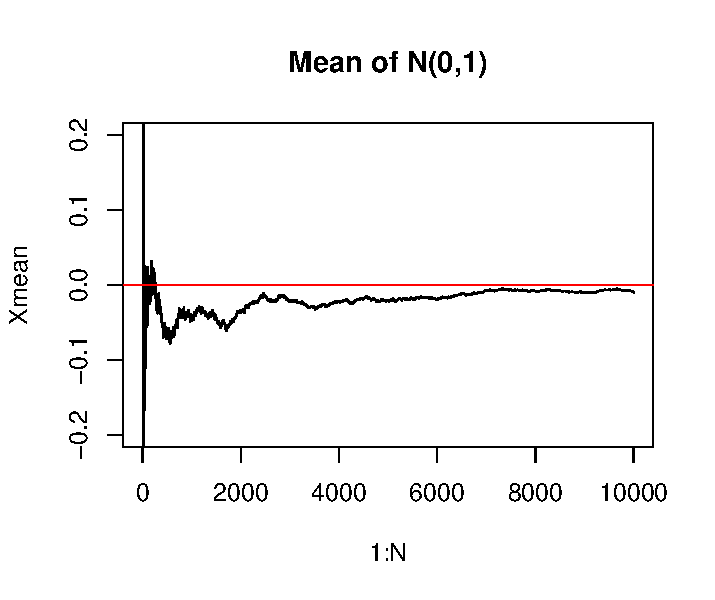
\includegraphics[scale=0.7]{ch3_3.9A.pdf}
        \end{figure}
    \end{center}
    \end{minipage}
    \begin{minipage}{0.5\textwidth}
    \begin{center}
        \begin{figure}[H]
            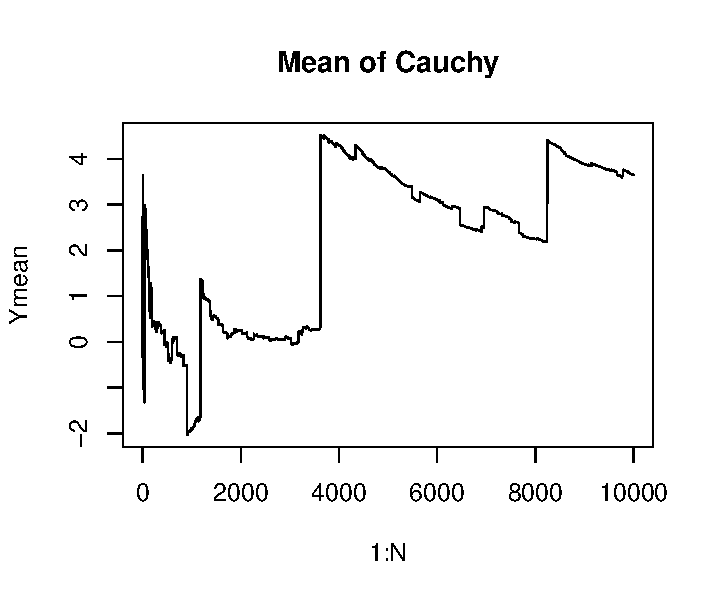
\includegraphics[scale=0.7]{ch3_3.9B.pdf}
        \end{figure}
    \end{center}
    \end{minipage}
\end{figure}

\begin{lstlisting}[style=RSyntax, title=R]
# Setting the number of simulations
N = 10000

# Simulating N standard normal values
X = rnorm(N)
Xmean = cumsum(X)/1:N
plot(1:N, Xmean, type="l", ylim = c(-0.2, 0.2),
main = "Mean of N(0,1)")
abline(h = 0, col="red")

# Simulating N Cauchy values with loc = 0, scale = 1
Y = rcauchy(N)
Ymean = cumsum(Y)/1:N
plot(1:N, Ymean, type="l",
main = "Mean of Cauchy")
\end{lstlisting}

\newpage\noindent
%%%%%%%%%%%%%%%%%%%%%%%%%%%%%%%%%%%%%%%%%%%%%%%%%%%%%%%%%%%%%%%%%%%%%%%%%%%%%%%
\textbf{3.10}\\  % PDF page 59
Let $X\sim N(0,1)$ and define $Y = e^X$. Find $\E[Y]$ and $\V(Y)$.

\medskip\noindent
One possible way to solve this is defining $r(X) = e^X$ and evaluating:
$$
\E[Y] = \E[r(X)] = \int_{\R} e^xf_X(x)dx
= \frac{1}{\sqrt{2\pi}}\int_{\R} \exp\left(x - \frac{1}{2}x^2\right)dx.
$$
Completing the square in the exponential term:
$$
x - \frac{1}{2}x^2 = -\frac{1}{2}\left(x^2 - 2x\right)
= -\frac{1}{2}\left(x^2 - 2x + 1 - 1\right)
= -\frac{1}{2}\left(x - 1\right)^2 + \frac{1}{2}
$$
We can rewrite the integral:
$$
\E[Y] = e^{1/2}\frac{1}{\sqrt{2\pi}}\int_{\R} \exp\left(-\frac{1}{2}(x - 1)^2\right)dx
$$
We will integrate this by substitution:
$$
u = x-1 \imp du/dx = 1 \imp du = dx
$$
$$
\E[Y] = e^{1/2}\underbrace{\frac{1}{\sqrt{2\pi}}\int_{\R} \exp\left(-\frac{1}{2}u^2\right)du}_{=1}
= e^{1/2} \approx 1.6487
$$
Confirming with numerical simulation.
\begin{lstlisting}[style=RSyntax]
> N = 10000000; X = rnorm(N); Y = exp(X)
> mean(Y)
[1] 1.648564
> exp(0.5)
[1] 1.648721
> var(Y)
[1] 4.676382
> exp(2) - exp(1)
[1] 4.670774
\end{lstlisting}
We can calculate the variance by first finding the second moment: $\E[Y^2]$.
$$
\E[Y^2] = \E[r(X)^2] = \int_{\R} e^{2x}f_X(x)dx
= \frac{1}{\sqrt{2\pi}}\int_{\R} \exp\left(2x - \frac{1}{2}x^2\right)dx.
$$
Just as above, we complete the square and get: $-(1/2)(x - 2)^2 + 2$ and move $e^2$ outside the integral. Then
we use integration by substitution: $u = x - 2$ which gives $du = dx$. We end up with a similar integral: 
$$
\E[Y^2] = e^{2}\underbrace{\frac{1}{\sqrt{2\pi}}\int_{\R} \exp\left(-\frac{1}{2}u^2\right)du}_{=1}
= e^{2}
$$
Now we can calculate the variance of $Y$.
$$
\V(Y) = \E[Y^2] - \E[Y]^2 = e^2 - (e^{1/2})^2 = e^2 - e^1,
$$
and as we can see in the simulation above, this corresponds to the simulated variance.

\newpage\noindent
%%%%%%%%%%%%%%%%%%%%%%%%%%%%%%%%%%%%%%%%%%%%%%%%%%%%%%%%%%%%%%%%%%%%%%%%%%%%%%%
\textbf{3.11}\\  % PDF page 59
Simulating stocks. For each day $Y_i$ can be either $-1$ or 1, each with probability 1/2.
We have $X_n = \sum_{i=1}^n Y_i$ which is the cumulative value of the stock.

\medskip\noindent(a) Calculating the expectation and variance of $X_n$. First we calculate it for
$Y_i$.
$$
\E[Y_i] = (-1)(1/2) + (1)(1/2) = -1/2 + 1/2 = 0
$$
$$
\E[Y_i^2] = (-1)^2(1/2) + (1)^2(1/2) = 1/2 + 1/2 = 1
$$
$$
\V(Y_i) = \E[Y_i^2] - \E[Y_i]^2 = 1 - 0 = 1
$$
Now for $X_n$.
$$
\E[X_n] = \E\left[\sum_{i=1}^n Y_i\right] = \sum_{i=1}^n \E[Y_i] = 0
$$
$$
\V(X_n) = \V\left[\sum_{i=1}^n Y_i\right] = \sum_{i=1}^n \V[Y_i] = \sum_{i=1}^n 1 = n
$$
(b) Simulating four stocks.
\begin{lstlisting}[style=RSyntax, title=R]
simStock <- function(N) {
    dailyMovements = sample(c(-1, 1), size=N, replace = TRUE)
    totalMovements = cumsum(dailyMovements)
    return(totalMovements)
} 
N = 10000
s1 = simStock(N);s2 = simStock(N)
s3 = simStock(N);s4 = simStock(N)
plot(1:N, s1, type="l",
    ylim=c(-119, 212), # Adjust according to simulation results
    main = "Stock simulation")
lines(1:N, s2, type="l", col="red")
lines(1:N, s3, type="l", col="blue")
lines(1:N, s4, type="l", col="green")
\end{lstlisting}
\begin{figure}[H]
    \begin{minipage}{0.55\textwidth}
        \begin{figure}[H]
            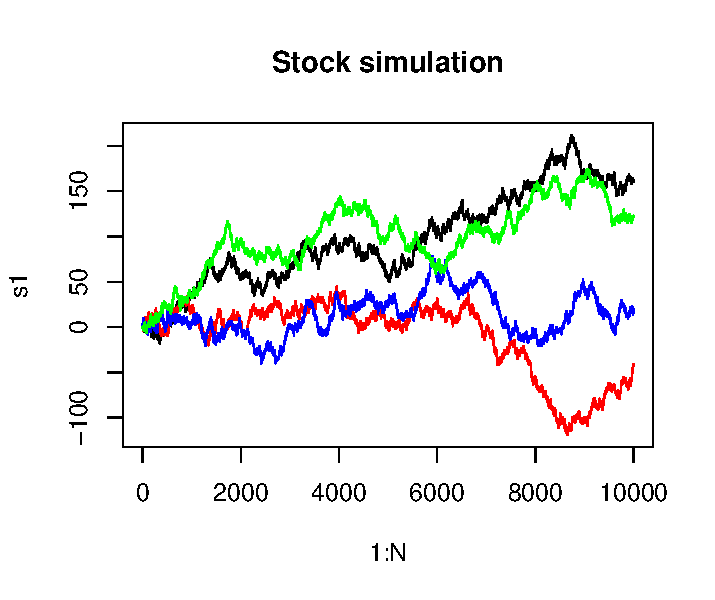
\includegraphics[scale=0.6]{ch3_11.pdf}
        \end{figure}
    \end{minipage}
    \begin{minipage}{0.45\textwidth}
        \medskip\noindent
        The simulations have mean 0, so they should vary around the x-axis.
        Since the variance is $n$, it is dependent on the time. The longer
        the simulations last, the more they will vary which is what we see.

        \medskip\noindent The standard deviation in this example will be
        the square root of $n$, which is about 100, and that is also what
        we see (and it is expected that they will not be exactly on the standard
        deviation).
    \end{minipage}
\end{figure}

\newpage\noindent
%%%%%%%%%%%%%%%%%%%%%%%%%%%%%%%%%%%%%%%%%%%%%%%%%%%%%%%%%%%%%%%%%%%%%%%%%%%%%%%
\textbf{3.12}\\  % PDF page 60
Deriving the general expression for the expectation and variance for a whole bunch of
probability distributions.

\medskip\noindent$\bullet$ \textbf{Bernoulli} with parameter $p$. Possible values: $\mc{X} = \{0, 1\}$.
$$
f(x) = p^x(1-p)^{x-1}
$$
Expectation.
$$
\E[X] = \sum_{x\in\mc{X}} x\cdot f(x) = (0) + (1)p^1 = p
$$
Second moment.
$$
\E[X^2] = \sum_{x^2\in\mc{X}} x^2\cdot f(x) = (0) + (1)^2p^1 = p
$$
Variance.
$$
\V(X) = \E[X^2] - \E[X]^2 = p - p^2 = p(1 - p)
$$

\medskip\noindent$\bullet$ \textbf{Poisson} with parameter $\lambda$. Possible values: $\mc{X} = \N\cup\{0\}$.
$$
f(x) = e^{-\lambda}\frac{\lambda^x}{x!}
$$
Expectation. First term disappears. Cancel $x$ against the factorial. Switch to $k = x-1$. 
\begin{align*}
    \E[X] &= \sum_{x\in\mc{X}} xf(x) = \sum_{x=0}^\infty x\cdot e^{-\lambda}\frac{\lambda^x}{x!} \\
    &= 0 + \lambda e^{-\lambda}\sum_{x=1}^\infty\frac{\lambda^{x-1}}{(x-1)!} \\
    &= \lambda e^{-\lambda}\sum_{k=0}^\infty\frac{\lambda^k}{k!} \\
    &= \lambda e^{-\lambda}e^{\lambda} \\
    &= \lambda
\end{align*}
Second moment. We will split the sum into two Poisson sums.
\begin{align*}
    \E[X^2] &=  \sum_{x^2\in\mc{X}} x^2\cdot f(x) = \sum_{x=0}^\infty x^2\cdot e^{-\lambda}\frac{\lambda^x}{x!} \\
    &= 0 + \lambda e^{-\lambda}\sum_{x=1}^\infty x\cdot \frac{\lambda^{x-1}}{(x-1)!} \\
    &= \lambda e^{-\lambda}\sum_{x=1}^\infty (x - 1 + 1)\cdot \frac{\lambda^{x-1}}{(x-1)!} \\
    &= \lambda e^{-\lambda}\sum_{x=1}^\infty\Big[(x - 1)\frac{\lambda^{x-1}}{(x-1)!} + \frac{\lambda^{x-1}}{(x-1)!}\Big]
\end{align*}

\newpage\noindent
\begin{align*}
    &= \lambda e^{-\lambda}\left(\sum_{x=2}^\infty(x - 1)\frac{\lambda^{x-1}}{(x-1)!} + 
    \sum_{x=1}^\infty\frac{\lambda^{x-1}}{(x-1)!}\right) \\
    &= \lambda e^{-\lambda}\left(\lambda\sum_{x=2}^\infty\frac{\lambda^{x-2}}{(x-2)!} + 
    \sum_{x=1}^\infty\frac{\lambda^{x-1}}{(x-1)!}\right) \\
    &= \lambda e^{-\lambda}\left(\lambda\sum_{j=0}^\infty\frac{\lambda^{j}}{j!} + 
    \sum_{k=0}^\infty\frac{\lambda^{k}}{k!}\right) \\
    &= \lambda e^{-\lambda}\left(\lambda e^{\lambda} + e^{\lambda}\right) \\
    &= \lambda^2 + \lambda
\end{align*}
The remaining calculation for the variance is easy.
$$
\V(X) = \E[X^2] - \E[X]^2 = \lambda^2 + \lambda - \lambda^2 = \lambda
$$

\medskip\noindent$\bullet$ \textbf{Uniform} on $(a, b)$. Possible values: $\mc{X} = (a,b)$. 
$$
f(x) = \frac{1}{b - a}
$$
Expectation.
\begin{align*}
    \E[X] &= \int_{\mc{X}} x\cdot f(x) = \frac{1}{b-a}\int_a^b x dx \\
    &= \frac{1}{b-a}\Big[\frac{x^2}{2}\Big]_a^b = \frac{1}{b-a}\left(\frac{b^2 - a^2}{2}\right) \\
    &= \frac{1}{b-a}\left(\frac{(b+a)(b-a)}{2}\right) \\
    &= \frac{b + a}{2}
\end{align*}
Second moment.
\begin{align*}
    \E[X^2] &= \int_{\mc{X}} x^2\cdot f(x) = \frac{1}{b-a}\int_a^b x^2 dx \\
    &= \frac{1}{b-a}\Big[\frac{x^3}{3}\Big]_a^b = \frac{1}{b-a}\left(\frac{b^3 - a^3}{3}\right) \\
    &= \frac{1}{b-a}\left(\frac{(b-a)(b^2 + ab + a^2)}{3}\right) \\
    &= \frac{b^2 + ab + a^2}{3}
\end{align*}
Variance.
\begin{align*}
    \V(X) &= \E[X^2] - \E[X]^2 = \frac{b^2 + ab + a^2}{3} - \frac{(b+a)^2}{4}\\ % = \frac{(b-a)^2}{12} \\
    &= \frac{4b^2 + 4ab + 4a^2 - 3b^2 - 6ab - 3a^2}{12} = \frac{b^2 - 2ab + a^2}{12} = \frac{(b-a)^2}{12}
\end{align*}

\newpage\noindent$\bullet$ \textbf{Exponential} with parameter $\beta$. Possible values: $\mc{X} = \{x\in\R : x\geq0\}$. 
$$
f(x) = \frac{1}{\beta}\exp(-x/\beta)
$$
Expectation.
\begin{align*}
    \E[X] &= \int_{\mc{X}} x\cdot f(x) = \int_0^\infty x\cdot \frac{1}{\beta} e^{-x/\beta} dx
\end{align*}
We will integrate this with the substitution $u = x/\beta$, so $du/dx = 1/\beta$ which gives us $dx = \beta du$.
Note that the antiderivative of $ue^{-u}$ is $-ue^{-u} - e^{-u}$.
\begin{align*}
    \E[X] &= \int_0^\infty x\cdot \frac{1}{\beta} e^{-x/\beta} dx
    = \beta\int_0^\infty u e^{-u} du \\
    &= \beta\Big[-ue^{-u} - e^{-u}\Big]_0^\infty \\
    &= \beta\Big(\lim_{u\ra\infty}(-ue^{-u} - e^{-u}) - (- 1)\Big) \\
    &= \beta
\end{align*}
    Skipping the evaluation of the limit. The first term can be shown to converge to 0 by using L'Hôpital's rule.
    The second term in the limit obviously becomes 0.\\
Second moment. Will derive the expression for the expectation in the calculations.
\begin{align*}
    \E[X^2] &= \int_{\mc{X}} x^2\cdot f(x) = \int_0^\infty x^2\cdot \frac{1}{\beta} e^{-x/\beta} dx
\end{align*}
Using integration by parts: $u = x^2$ so $u' = 2x$. Setting $v' = (1/\beta)e^{-x/\beta}$ which yields
$v = -e^{-x/\beta}$. From the integration-by-parts formula:
$$
\int uv' = uv - \int u'v
$$
\begin{align*}
    \E[X^2] = \int_0^\infty x^2\cdot \frac{1}{\beta} e^{-x/\beta} dx
    &= \Big[-x^2e^{-x/\beta}\Big]_0^\infty - \int_0^\infty -2x e^{-x/\beta}dx \\
    &= 0 + \int_0^\infty 2x e^{-x/\beta}dx  \\
    &= 2\beta\int_0^\infty x\cdot\frac{1}{\beta}e^{-x/\beta}dx  \\
    &= 2\beta\E[X] \\
    &= 2\beta^2
\end{align*}
The limit can be shown to converge to 0 by applying L'Hôpital's rule twice. We use a clever trick and
substitute in the expectation and get the result. Finally, we calculate the variance.
$$
\V(X) = \E[X^2] - \E[X]^2 = 2\beta^2 - \beta^2 = \beta^2
$$
\newpage\noindent$\bullet$ \textbf{Gamma} with parameters $\alpha,\beta$.
Possible values: $\mc{X} = \{x\in\R : x > 0\}$. 
$$
f(x) = \frac{1}{\Gamma(\alpha)\beta^\alpha}x^{\alpha-1}\exp(-x/\beta)
$$
We will use the definition of the Gamma function, and the 'Gamma difference' chaining property:
$$
\Gamma(\alpha+1) = \int_0^\infty t^{\alpha}e^{-t}dt,\quad
\Gamma(\alpha+1) = \alpha\Gamma(\alpha)
$$
In step 3, we make the substitution $t = x/\beta$ which makes $x = \beta t$.
$dt/dx = 1/\beta$, so $dx = \beta dt$.
\begin{align*}
    \E[X] &= \int_{\mc{X}} x\cdot f(x)
    = \int_0^\infty x\cdot\frac{1}{\Gamma(\alpha)\beta^\alpha}x^{\alpha-1}\exp(-x/\beta) dx \\
    &= \int_0^\infty \frac{1}{\Gamma(\alpha)\beta^\alpha}x^{\alpha}\exp(-x/\beta) dx \\
    &= \int_0^\infty \frac{1}{\Gamma(\alpha)\beta^\alpha}(\beta t)^{\alpha}\exp(-t) \beta dt\\
    &= \int_0^\infty \frac{1}{\Gamma(\alpha)\beta^\alpha}\beta^\alpha t^{\alpha}\exp(-t) \beta dt\\
    &= \int_0^\infty \frac{1}{\Gamma(\alpha)\beta^\alpha}\beta^{\alpha+1} t^{\alpha}\exp(-t) dt\\
    &= \frac{\beta^{\alpha+1}}{\Gamma(\alpha)\beta^\alpha}\int_0^\infty t^{\alpha}\exp(-t) dt\\
    &= \frac{\beta}{\Gamma(\alpha)}\int_0^\infty t^{\alpha}\exp(-t) dt\\
    &= \frac{\beta\Gamma(\alpha + 1)}{\Gamma(\alpha)}\\
    &= \frac{\beta\alpha\Gamma(\alpha)}{\Gamma(\alpha)}\\
    &= \alpha\beta
\end{align*}
For the Gamma distribution, we will not calculate the second moment. Instead we will go straight to the
variance calculation and calculate it directly. We will use the same substitution and use the definition of
the Gamma function again.
\begin{align*}
    \V(X) = \E[X^2] - \E[X]^2 &= 
    \int_0^\infty x^2\cdot\frac{1}{\Gamma(\alpha)\beta^\alpha}x^{\alpha-1}\exp(-x/\beta) dx - \alpha^2\beta^2 \\
    &= \frac{1}{\Gamma(\alpha)\beta^\alpha}\int_0^\infty x^{\alpha+1}\exp(-x/\beta) dx - \alpha^2\beta^2 \\
    &= \frac{1}{\Gamma(\alpha)\beta^\alpha}\int_0^\infty (\beta t)^{\alpha+1}\exp(-t) \beta dt - \alpha^2\beta^2 \\
    &= \frac{\beta^{\alpha+2}}{\Gamma(\alpha)\beta^\alpha}\int_0^\infty t^{\alpha+1}\exp(-t) dt - \alpha^2\beta^2 
\end{align*}

\newpage\noindent
Using the definition of the Gamma function.
\begin{align*}
    &= \frac{\beta^{2}\Gamma(\alpha + 2)}{\Gamma(\alpha)} - \alpha^2\beta^2 \\
    &= \frac{\beta^{2}\Gamma(\alpha + 2) - \alpha^2\beta^2\Gamma(\alpha)}{\Gamma(\alpha)} \\
    &= \frac{\beta^{2}\big(\Gamma(\alpha + 2) - \alpha^2\Gamma(\alpha)\big)}{\Gamma(\alpha)} \\
    &= \frac{\beta^{2}\big((\alpha + 1)\Gamma(\alpha + 1) - \alpha^2\Gamma(\alpha)\big)}{\Gamma(\alpha)} \\
    &= \frac{\beta^{2}\big((\alpha + 1)\alpha\Gamma(\alpha) - \alpha^2\Gamma(\alpha)\big)}{\Gamma(\alpha)} \\
    &= \frac{\beta^{2}\Gamma(\alpha)\big((\alpha + 1)\alpha - \alpha^2\big)}{\Gamma(\alpha)} \\
    &= \beta^{2}\big((\alpha + 1)\alpha - \alpha^2\big)\\
    &= \beta^{2}\big(\alpha^2 \alpha - \alpha^2\big) \\
    &= \alpha\beta^2
\end{align*}
And the calculation for the Gamma distribution has been completed.

\bigskip\noindent$\bullet$ \textbf{Beta} with parameter $\alpha,\beta$. Possible values: $\mc{X} = (0,1)$. 
$$
f(x) = \frac{\Gamma(\alpha + \beta)}{\Gamma(\alpha)\Gamma(\beta)}x^{\alpha - 1}(1 - x)^{\beta-1}
$$
In the following, we will use the following definition:
$$
\frac{\Gamma(\alpha)\Gamma(\beta)}{\Gamma(\alpha + \beta)} =
\int_0^1 t^{\alpha - 1}(1 - t)^{\beta - 1}dt
$$
Expectation.
\begin{align*}
    \E[X] &= \int_{\mc{X}} x\cdot f(x) = \int_0^1 x\cdot\frac{\Gamma(\alpha + \beta)}{\Gamma(\alpha)\Gamma(\beta)}x^{\alpha - 1}(1 - x)^{\beta-1} dx\\
    &= \frac{\Gamma(\alpha + \beta)}{\Gamma(\alpha)\Gamma(\beta)}\int_0^1 x^{\alpha}(1 - x)^{\beta-1} dx\\
    &= \frac{\Gamma(\alpha + \beta)}{\Gamma(\alpha)\Gamma(\beta)}\cdot\frac{\Gamma(\alpha + 1)\Gamma(\beta)}{\Gamma(\alpha + \beta + 1)} \\
    &= \frac{\Gamma(\alpha + \beta)}{\Gamma(\alpha)\Gamma(\beta)}\cdot\frac{\alpha\Gamma(\alpha)\Gamma(\beta)}{(\alpha + \beta)\Gamma(\alpha + \beta)}\\
    &= \frac{\alpha}{\alpha + \beta}\cdot\frac{\Gamma(\alpha + \beta)}{\Gamma(\alpha)\Gamma(\beta)}\cdot\frac{\Gamma(\alpha)\Gamma(\beta)}{\Gamma(\alpha + \beta)}\\
    &= \frac{\alpha}{\alpha + \beta}
\end{align*}
\newpage\noindent
Variance. Just like for the Gamma distribution, we calculate the second moment directly in the variance
calculation. Will use a lot of the same tricks as when calculating the expectation.
\begin{align*}
    \V(X) = \E[X^2] - \E[X]^2 &= 
    \int_0^1 x^2\cdot\frac{\Gamma(\alpha + \beta)}{\Gamma(\alpha)\Gamma(\beta)}x^{\alpha - 1}(1 - x)^{\beta-1}dx - \left(\frac{\alpha}{\alpha + \beta}\right)^2 \\
    &= \frac{\Gamma(\alpha + \beta)}{\Gamma(\alpha)\Gamma(\beta)}\int_0^1 x^{\alpha + 1}(1 - x)^{\beta-1}dx - \left(\frac{\alpha}{\alpha + \beta}\right)^2 \\
    &= \frac{\Gamma(\alpha + \beta)}{\Gamma(\alpha)\Gamma(\beta)}\int_0^1 x^{\alpha + 1}(1 - x)^{\beta-1}dx - \left(\frac{\alpha}{\alpha + \beta}\right)^2\\
    &= \frac{\Gamma(\alpha + \beta)}{\Gamma(\alpha)\Gamma(\beta)}\cdot\frac{\Gamma(\alpha + 2)\Gamma(\beta)}{\Gamma(\alpha + \beta + 2)} - \left(\frac{\alpha}{\alpha + \beta}\right)^2 \\
    &= \frac{\alpha(\alpha + 1)}{(\alpha + \beta)(\alpha + \beta + 1)}\cdot\frac{\Gamma(\alpha + \beta)}{\Gamma(\alpha)\Gamma(\beta)}\cdot\frac{\Gamma(\alpha)\Gamma(\beta)}{\Gamma(\alpha + \beta)} - \left(\frac{\alpha}{\alpha + \beta}\right)^2 \tag{3.12.1} \\
    &= \frac{\alpha(\alpha + 1)}{(\alpha + \beta)(\alpha + \beta + 1)} - \left(\frac{\alpha}{\alpha + \beta}\right)^2 \\
    &= \frac{\alpha^2 + \alpha}{(\alpha + \beta)(\alpha + \beta + 1)} - \frac{\alpha^2}{(\alpha + \beta)^2} \\
    &= \frac{(\alpha^2 + \alpha)(\alpha + \beta) - \alpha^2(\alpha + \beta + 1)}{(\alpha + \beta)^2(\alpha + \beta + 1)} \\
    &= \frac{\alpha^3 + \alpha^2\beta + \alpha^2 + \alpha\beta - \alpha^3 - \alpha^2\beta - \alpha^2)}{(\alpha + \beta)^2(\alpha + \beta + 1)} \\
    &= \frac{\cancel{\alpha^3} + \cancel{\alpha^2\beta} + \cancel{\alpha^2} + \alpha\beta \cancel{- \alpha^3} \cancel{- \alpha^2\beta} \cancel{- \alpha^2})}{(\alpha + \beta)^2(\alpha + \beta + 1)} \\
    &= \frac{\alpha\beta}{(\alpha + \beta)^2(\alpha + \beta + 1)}
\end{align*}
In step (3.12.1) we used the difference/chaining property of the Gamma function.
$$
\Gamma(\alpha + 2) = (\alpha + 1)\Gamma(\alpha + 1) = (\alpha + 1)\alpha\Gamma(\alpha)
$$
and,
$$
\Gamma(\alpha + \beta + 2) = (\alpha + \beta + 1)\Gamma(\alpha + \beta + 1) =
(\alpha + \beta + 1)(\alpha + \beta)\Gamma(\alpha + \beta)
$$
This concludes the last calculation. I found this exercise to be a little tedious, to be honest...

\bigskip\noindent
%%%%%%%%%%%%%%%%%%%%%%%%%%%%%%%%%%%%%%%%%%%%%%%%%%%%%%%%%%%%%%%%%%%%%%%%%%%%%%%
\textbf{3.13}\\  % PDF page 60
A variable $X$ is generated by assuming a value in $U(0,1)$ if a coin toss
is 0 (H), and $X$ is in $U(3,4)$ if the coin toss is 1 (T). The coin is fair, so
each of these has a probability of 1/2.

\medskip\noindent(a) Calculating the mean of $X$. This will be a conditional expectation,
and we define $Y$ to be the coin toss. The marginal distributions might depend on the outcome,
but when we calculate them:
$$
f_{X|Y}(x|Y=0) = \frac{1}{1-0} = 1, \quad
f_{X|Y}(x|Y=1) = \frac{1}{4-3} = 1,
$$
we find that it will be $f_{X|Y}(x|y) = 1$ either way.

\newpage\noindent
Now we can calculate the expected value for specific outcomes.
$$
\E[X|Y=0] =  \int_{\mc{X}}x\cdot f_{X|Y}(x|y) = \int_0^1 x dx = \left[\frac{x^2}{2}\right]_0^1 = \frac{1-0}{2} = \frac{1}{2}
$$
$$
\E[X|Y=1] = \int_{\mc{X}}x\cdot f_{X|Y}(x|y) = \int_3^4 x dx = \left[\frac{x^2}{2}\right]_3^4 = \frac{16-9}{2} = \frac{7}{2}
$$
Using that $p_Y(y)$ is known, we can calculate the expected value of $X$:
\begin{align*}
    \E[X] = \E[\E[X|Y]] &= \sum_{y\in\{0,1\}}\E[X|Y=y]\P(Y=y) \\
    &= \left(\frac{1}{2}\right)\left(\frac{1}{2}\right) + \left(\frac{7}{2}\right)\left(\frac{1}{2}\right) \\
    &= \frac{1}{4} + \frac{7}{4} = \frac{8}{4} = 2
\end{align*}
% (b) Calculating the variance. We can do a direct calculation with the definition of the conditional variance.
% \begin{align*}
%     \V(X|Y=y) &= \int_0^1(x - 1/2)^2 dx + \int_3^4(x - 7/2)^2 dx \\
%     &= \int_0^1(x^2 - x + 1/4) dx + \int_3^4(x^2 - 7x + 49/4) dx \\
%     &= \Big[\frac{x^3}{3} - \frac{x^2}{2} + \frac{x}{4}\Big]_0^1 + \Big[\frac{x^3}{3} - \frac{7x^2}{2} + \frac{49}{4}\Big]_3^4 \\
%     &= \frac{1}{12}
% \end{align*}
(b) Calculating the second moment.
$$
\E[X^2|Y=0] =  \int_{\mc{X}}x^2\cdot f_{X|Y}(x|y) = \int_0^1 x^2 dx = \left[\frac{x^3}{3}\right]_0^1 = \frac{1-0}{3} = \frac{1}{3}
$$
$$
\E[X^2|Y=1] = \int_{\mc{X}}x^2\cdot f_{X|Y}(x|y) = \int_3^4 x^2 dx = \left[\frac{x^3}{3}\right]_3^4 = \frac{4^3-3^3}{3} = \frac{37}{3}
$$
\begin{align*}
    \E[X^2] = \E[\E[X^2|Y]] &= \sum_{y\in\{0,1\}}\E[X^2|Y=y]\P(Y=y) \\
    &= \left(\frac{1}{3}\right)\left(\frac{1}{2}\right) + \left(\frac{37}{3}\right)\left(\frac{1}{2}\right) \\
    &= \frac{1}{6} + \frac{37}{6} = \frac{38}{6} \\
    &= \frac{19}{3}
\end{align*}
Calculating the variance:
$$
\V(X) = \E[X^2] - \E[X]^2 = \frac{19}{3} - 4 = \frac{7}{3} \approx 2.333
$$
And finally the standard deviation:
$$
\text{SD}(X) = \sqrt{\V(X)} = \sqrt{\frac{7}{3}} \approx 1.5275
$$
To verify these results, we did a numeric simulation.

\newpage\noindent
\begin{lstlisting}[style=RSyntax, title=R]
N = 10000; Y = sample(c(0, 1), size=N, replace = TRUE); X = rep(0, N)
for (i in 1:N) {
    if (Y[i] == 1) X[i] = runif(1)
    else X[i] = runif(1, min=3, max=4) 
}   
> mean(X)
[1] 2.01424
> var(X)
[1] 2.332699
> sd(X)
[1] 1.527318
\end{lstlisting}

\medskip\noindent
%%%%%%%%%%%%%%%%%%%%%%%%%%%%%%%%%%%%%%%%%%%%%%%%%%%%%%%%%%%%%%%%%%%%%%%%%%%%%%%
\textbf{3.14}\\  % PDF page 60
\textbf{Claim}: Let $X_1,\ldots, X_m$ and $Y_1,\ldots, Y_n$ be random variables and
$a_1,\ldots, a_m$ and $b_1,\ldots, b_n$ be constants. Then:
$$
\Cov\left(\sum_{i=1}^m a_iX_i, \sum_{j=1}^n b_iY_i\right)
= \sum_{i=1}^m\sum_{j=1}^n a_ib_j \Cov(X_i, Y_j).
$$
\textsc{Proof}. This can be verified with a direct proof. We will do a simplified example
with $m = n = 2$, which is not a formal proof, but can easily be extended to one. We will repeatedly use:
$$
\Cov(A, B) = \E[AB] - \E[A]\E[B].
$$
Starting with the covariance, we apply the identity above. We have, for $m=n=2$:
\begin{align*}
\Cov(a_1X_1 + a_2X_2, b_1Y_1 + b_2Y_2) &=
\E[(a_1X_1 + a_2X_2)(b_1Y_1 + b_2Y_2)] - \E[a_1X_1 + a_2X_2]\E[b_1Y_1 + b_2Y_2] \\
&= S_1 - S_2
\end{align*}
Multiplying and rewriting the first term:
\begin{align*}
    S_1 = \E[(a_1X_1 + a_2X_2)(b_1Y_1 + b_2Y_2)] &=
    \E[a_1b_1X_1Y_1 + a_1b_2X_1Y_2 + a_2b_1X_2Y_1 + a_2b_2X_2Y_2] \\
    &= a_1b_1\E[X_1Y_1] + a_1b_2\E[X_1Y_2] + a_2b_1\E[X_2Y_1] + a_2b_2\E[X_2Y_2]
\end{align*}
The second term:
\begin{align*}
    S_2 = \E[a_1X_1 + a_2X_2]\E[b_1Y_1 + b_2Y_2] &= \left(a_1\E[X_1] + a_2\E[X_2]\right)\left(b_1\E[Y_1] + b_2\E[Y_2]\right) \\
    &= a_1b_1\E[X_1]\E[Y_1] + a_1b_2\E[X_1]\E[Y_2] + a_2b_1\E[X_2]\E[Y_1] + a_2b_2\E[X_2]\E[Y_2]
\end{align*}
Subtracting:
\begin{align*}
    S_1 - S_2 &= a_1b_1\E[X_1Y_1] + a_1b_2\E[X_1Y_2] + a_2b_1\E[X_2Y_1] + a_2b_2\E[X_2Y_2] \\
    &\;\;- a_1b_1\E[X_1]\E[Y_1] - a_1b_2\E[X_1]\E[Y_2] - a_2b_1\E[X_2]\E[Y_1] - a_2b_2\E[X_2]\E[Y_2] \\
    &= a_1b_1(\E[X_1Y_1] - \E[X_1]\E[Y_1]) + a_1b_2(\E[X_1Y_2] - \E[X_1]\E[Y_2]) \\
    &\;\; + a_2b_1(\E[X_2Y_1] - \E[X_2]\E[Y_1]) + a_2b_2(\E[X_2Y_2] - \E[X_2]\E[Y_2]) \\
    &= a_1b_1\Cov(X_1, Y_1) + a_1b_2\Cov(X_1, Y_2) + a_2b_1\Cov(X_2, Y_1) + a_2b_2\Cov(X_2, Y_2) \\
    &= \sum_{i=1}^2\sum_{i=j}^2 a_ib_j\Cov(X_i, Y_j) \tag*{\qed}
\end{align*}

\newpage\noindent
%%%%%%%%%%%%%%%%%%%%%%%%%%%%%%%%%%%%%%%%%%%%%%%%%%%%%%%%%%%%%%%%%%%%%%%%%%%%%%%
\textbf{3.15}\\  % PDF page 60
Defining the joint distribution:
$$
f_{X,Y}(x,y) =
\left\{
    \begin{tabular}{ll}
        $\displaystyle \frac{1}{3}(x + y)$ & $0\leq x\leq 1, 0\leq y\leq 2$ \\
        $0$\rule{0pt}{15pt} & otherwise
    \end{tabular}
\right.
$$
We will calculate $\V(2X - 3Y + 8)$. Constants disappear in the variance, and by Theorem 2.30:
$$
\V(2X - 3Y + 8) = 4\V(X) + 9\V(Y) - 12\Cov(X, Y) 
$$
Finding the marginal distributions:
$$
f_X(x) = \int_0^2 \frac{1}{3}x + \frac{1}{3}y dy = \Big[ \frac{1}{3}xy + \frac{1}{6}y^2 \Big]_0^2
= \frac{2x}{3} + \frac{2}{3}
$$
$$
f_Y(y) = \int_0^1 \frac{1}{3}x + \frac{1}{3}y dx = \Big[ \frac{1}{6}x^2 + \frac{1}{3}xy \Big]_0^1
= \frac{y}{3} + \frac{1}{6} 
$$
Calculating the expectation of $X$.
$$
\E[X] = \int_0^1x\left(\frac{2x}{3} + \frac{2}{3}\right)dx
= \int_0^1\left(\frac{2x^2}{3} + \frac{2x}{3}\right)dx
= \left[\frac{2x^3}{9} + \frac{2x^2}{6}\right]_0^1 = \frac{5}{9}
$$
Second moment:
$$
\E[X^2] = \int_0^1x^2\left(\frac{2x}{3} + \frac{2}{3}\right)dx
= \int_0^1\left(\frac{2x^3}{3} + \frac{2x^2}{3}\right)dx
= \left[\frac{2x^4}{12} + \frac{2x^3}{9}\right]_0^1 = \frac{7}{18}
$$
Variance of $X$:
$$
\V(X) = \E[X^2] - \E[X]^2 = \frac{7}{18} - \frac{25}{81} = \frac{13}{162}
$$
Calculating the expectation of $Y$.
$$
\E[Y] = \int_0^2y\left(\frac{y}{3} + \frac{1}{6} \right)dy
= \int_0^2\left(\frac{y^2}{3} + \frac{y}{6} \right)dx
= \left[\frac{y^3}{9} + \frac{y^2}{12}\right]_0^2 = \frac{11}{9}
$$
Second moment:
$$
\E[Y^2] = \int_0^2y^2\left(\frac{y}{3} + \frac{1}{6} \right)dy
= \int_0^2\left(\frac{y^3}{3} + \frac{y^2}{6} \right)dx
= \left[\frac{y^4}{12} + \frac{y^3}{18}\right]_0^2 = \frac{16}{9}
$$
Variance of $Y$:
$$
\V(Y) = \E[Y^2] - \E[Y]^2 = \frac{16}{9} - \frac{121}{81} = \frac{23}{81}
$$

\newpage\noindent
From the definition of the covariance - these calculations are pretty large, so skipping the details:
\begin{align*}
    \Cov(X, Y) &= \E[(X-\E[X])(Y - \E[Y])] \\
    &= \int_0^2\int_0^1 \left(x - \frac{5}{9}\right)\left(y - \frac{11}{9}\right)\left(\frac{x}{3} + \frac{y}{3}\right)dxdy\\
    &= \frac{1}{486}\int_0^2 -9y^2 + 20y - 11 dy \\
    &= - \frac{1}{81}
\end{align*}
Putting it all together:
\begin{align*}
    \V(2X + 3Y - 8) &= 4\V(X) + 9\V(Y) - 12\Cov(X, Y) \\
    &= 4\left(\frac{13}{162}\right) + 9\left(\frac{23}{81}\right) - 12\left(-\frac{1}{81}\right) \\
    &= \frac{52}{162} + \frac{207}{81} + \frac{12}{81} \;=\; \frac{26}{81} + \frac{207}{81} + \frac{12}{81} \\
    &= \frac{245}{81}
\end{align*}

\bigskip\noindent
%%%%%%%%%%%%%%%%%%%%%%%%%%%%%%%%%%%%%%%%%%%%%%%%%%%%%%%%%%%%%%%%%%%%%%%%%%%%%%%
\textbf{3.16}\\  % PDF page 60
Let $r(x)$ and $s(y)$ be functions of $x$ and $y$. Then:
$$
\E[r(X)s(Y)|X] = r(X)\E[s(Y)|X], \qquad \E[r(X)|X] = r(X)
$$
\textsc{Proof}. By definition of the conditional expectation in the continuous case.
\begin{align*}
    \E[r(X)s(Y)|X=x] &= \int_{\mc{Y}} r(x)s(y)f_{Y|X}(y) dy \\
    &= r(x)\int_{\mc{Y}} s(y)f_{Y|X}(y) dy \\
    &= r(X)\E[s(Y)|X]
\end{align*}
For the special case, we can set $s(Y) = 1$.
\begin{align*}
    \E[r(X)|X=x] &= \int_{\mc{Y}} r(x)(1)f_{Y|X}(y) dy \\
    &= r(x)\int_{\mc{Y}} (1)f_{Y|X}(y) dy \\
    &= r(X)\E[(1)|X] \\
    &= r(X)
\end{align*}
which proves the statement. It is similar in the discrete case. \qed

% \newpage\noindent
% %%%%%%%%%%%%%%%%%%%%%%%%%%%%%%%%%%%%%%%%%%%%%%%%%%%%%%%%%%%%%%%%%%%%%%%%%%%%%%%
% \textbf{3.17}\\  % PDF page 60
% Proving that
% $$
% \V(Y) = \E[\V(Y|X)] + \V(\E[Y|X]).
% $$
% \textsc{Proof}.




\begin{comment}

\bigskip\noindent
%%%%%%%%%%%%%%%%%%%%%%%%%%%%%%%%%%%%%%%%%%%%%%%%%%%%%%%%%%%%%%%%%%%%%%%%%%%%%%%
\textbf{3.1X}\\  % PDF page 60


\begin{align*}
    A &= B
\end{align*}


\begin{equation*}
    A = B
    \tag*{\qed}
\end{equation*}


\begin{lstlisting}[style=RSyntax, title=R]
# Code
\end{lstlisting}

\begin{verbatim}
# Output
\end{verbatim}






%%%%%%%%%%%%%%%%%%%%%%%%%%%%%%%%%%%%%%%%%%% Minipages x 2
\begin{figure}[H]
    \begin{minipage}{0.5\textwidth}
        % MINIPAGE 1
    \end{minipage}
    \begin{minipage}{0.5\textwidth}
        % MINIPAGE 2
    \end{minipage}
\end{figure}

%%%%%%%%%%%%%%%%%%%%%%%%%%%%%%%%%%%%%%%%%%% Two R images
\begin{figure}[H]
    \begin{minipage}{0.5\textwidth}
    \begin{center}
        \begin{figure}[H]
            \includegraphics[scale=0.7]{IMG1.pdf}
        \end{figure}
    \end{center}
    \end{minipage}
    \begin{minipage}{0.5\textwidth}
    \begin{center}
        \begin{figure}[H]
            \includegraphics[scale=0.7]{IMG2.pdf}
        \end{figure}
    \end{center}
    \end{minipage}
\end{figure}


%%%%%%%%%%%%%%%%%%%%%%%%%%%%%%%%%%%%%%%%%%% Two TikZ images
%%% Tikz Image - side by side
\begin{figure}
    \begin{minipage}[0.5\textwidth]
\begin{tikzpicture}
    \begin{axis}[
        width=\textwidth,
        axis lines = left,
        ymin = -0.002,
        ymax = 2.1,
        xlabel = $z$,
        ylabel = {$f_Z(z)$},
    ]
    %Section 1
    \addplot [
        domain=0:1, 
        samples=10, 
        color=blue,
        style=ultra thick,
    ]
    {2 - 2*x};
    \end{axis}
\end{tikzpicture}
    \end{minipage}
    \begin{minipage}[0.5\textwidth]
\begin{tikzpicture}
    \begin{axis}[
        width=\textwidth,
        axis lines = left,
        ymin = -0.002,
        ymax = 2.1,
        xlabel = $z$,
        ylabel = {$f_Z(z)$},
    ]
    %Section 1
    \addplot [
        domain=0:1, 
        samples=10, 
        color=blue,
        style=ultra thick,
    ]
    {2 - 2*x};
    \end{axis}
\end{tikzpicture}
    \end{minipage}
\end{figure}



\end{comment}